\chapter{Cross section measurement for top quark pair production in association with a W or Z boson
in proton--proton collisions at $\sqrt{s}=\SI{13}{TeV}$}
\label{chap:13-TeV}
This chapter presents measurements of the \ttW and \ttZ cross sections performed using
\SI{35.9}{fb^{-1}} of \SI{13}{\TeV} pp collision data from the LHC. As in the analysis described
in~\cref{chap:8-TeV}, \ttW and \ttZ events were targeted where the associated boson produces
electrons or muons. The theoretical \ttW and \ttZ cross sections at \SI{13}{TeV} are \numrange{3}{4}
times higher than at \SI{8}{TeV}. This, combined with the higher integrated luminosity permitted a
more precise measurement to be made, while simplifying some aspects: the OS \ttZ and 3\lep \ttW
channels present in the earlier analysis were not targeted, a full event reconstruction is not
carried out, and a BDT was used only in the SS \ttW channel.

The reinterpretation of this measurement within the context of effective field theory is described
in~\cref{chap:eft}.

\section{Samples}
The data-driven estimation of backgrounds due to nonprompt leptons relies on control regions of data
collected, with single lepton triggers requiring the presence of at least one electron or muon with
$\pT > \SI{27}{GeV}$ or $\pT > \SI{24}{GeV}$. To simplify the treatment of this background, data
collected with the same triggers were used for signal regions. The trigger efficiencies exceeded
\SI{95}{\percent} for the SS \ttW channel and \SI{98}{\percent} for the 3\lep and 4\lep \ttZ
channels.

Expected signal events and some backgrounds were modeled with MC simulation. The simulated datasets
and their cross sections are summarized in~\cref{tab:13-samples}. The samples produced at LO in QCD
used the NNPDF3.0LO~\cite{Ball:2014uwa} PDF, while those at NLO in QCD used the
NNPDF3.0NLO~\cite{Ball:2014uwa} PDF. Parton showering, hadronization, and the underlying event were
simulated using \pythia~v8.212~\cite{Sjostrand:2007gs,Sjostrand:2014zea} with the CUETP8M1
tune~\cite{Skands:2014pea,CMS-PAS-GEN-14-001}. \geant software~\cite{Agostinelli:2002hh} was used to
model the CMS detector response. The pileup distribution was simulated to match the one observed in
the data.

\begin{table}
  \centering
  \input{tables/thirteen-TeV/samples}
\end{table}

\section{Event selection}
\label{section:13_event_selection}
We searched for \ttW and \ttZ events by optimizing the selection process for three exclusive final
states: SS \ttW, 3\lep \ttZ, and 4\lep \ttZ. These final states were described
in~\cref{section:8-event-selection} and have the same backgrounds and similar selection criteria.
The selection criteria for each final state are summarized in~\cref{tab:13-event-selection}. Each
channel was divided into categories according to the number of jets and b-tagged jets, and for the
SS \ttW channel, additionally according to the score from a BDT and the lepton charges. The \ttW BDT
and categorization scheme for each channel are described in more detail below.

\begin{table}
  \centering
  \caption{Summary of selection requirements for each channel}
  \label{tab:13-event-selection}
  \input{tables/thirteen-TeV/event-selection}
\end{table}

BDTs were described in~\cref{section:8_signal}. In the SS \ttW channel, a BDT with gradient
boosting~\cite{bdt_nim} is used to help distinguish signal \ttW events from backgrounds. The BDT is
trained with events from MC \ttW and \ttbar samples, divided into equal samples for training and
testing. The following variables were used as inputs: the number of jets, \njets; the number of b
jets, \nbjets; the scalar sum of \pT of the jets, \HT; \pTmiss; the highest-\pT (leading) and the
lowest-\pT (trailing) lepton \pT; the invariant mass calculated using \pTmiss and \pT of each
lepton, \MT; the highest (leading) and second highest (subleading) jet \pT; and the separation
$\Delta R$ between the trailing lepton and the nearest selected jet.

Events were divided into categories according to the BDT output score: $D < 0$ was used as a control
region to constrain uncertainties, and the signal region is divided into $0 < D < 0.6$ and $D >
0.6$. These definitions were determined to provide the optimal expected sensitivity. Signal region
events were additionally categorized according to whether they had two, three, or more than three
jets; those with three or more jets were further divided according to whether they had one or more
than one b-tagged jet. Because we are studying pp collisions, there is a charge asymmetry between
$\ttW^+$ and $\ttW^-$ production, while the majority of the backgrounds produce charge-symmetric
dileptons. We took advantage of this circumstance by further splitting the $D>0$ events according to
the lepton charge ($\ell^+\ell^+$ or $\ell^-\ell^-$).

In the 3\lep \ttZ channel, events were divided into nine exclusive categories: events with two,
three, or more than three jets, with each jet multiplicity being further split according to whether
it had zero, one, or more than one b tag. The two jet category provided a background-dominated
control region, which constrained uncertainties. Although signal \ttZ events have at least four
jets, we found that the expected sensitivity was improved by including the three-jet categories,
which have larger background contamination but allow for the recovery of events with merged jets or
jets that fall outside the acceptance limits.

Events in the 4\lep \ttZ channel were categorized according to whether they contained zero or at
least one b-tagged jet.

\section{Event modeling}
The background sources were described in~\cref{sec:8-modeling}. The modeling for each background is described below.

\subsection{Nonprompt backgrounds}
\label{ssec:13-TeV-nonprompt}
We used a data-based \emph{tight-to-loose} method to model background from nonprompt leptons
(introduced in~\cref{ssec:leptons}), which are an important background source in the SS \ttW and
3\lep channels.

We measured the rate\footnote{Note this rate is similar to $f$ measured using a modified
tag-and-probe technique and used in the \eightTeV analysis as described
in~\cref{ssec:8-TeV-nonprompt}. The different terminology is used to emphasize the different
definitions involved.} $f_\text{TL}$ at which loose leptons (see~\cref{tab:13-TeV-leptons}) also
pass the tight criteria in a multijet control region enriched with nonprompt leptons (the
\emph{measurement region}). We selected events with a single lepton and one or more jets, where the
lepton and jets were separated by $\Delta R > 1$. Contamination from prompt leptons (mainly from
W$+$jets) was suppressed by requiring $\pTmiss<\SI{20}{GeV}$ and $\MT<\SI{20}{GeV}$; any remaining
contamination (with a maximum contribution on the order of a few percent for high-\pT leptons) was
estimated from the simulation and subtracted.

Once $f_\text{TL}$ was obtained, it was applied to a second control region (the \emph{application}
region). In the application region, events must pass the full selection criteria except that one
lepton fails the tight selection but passes the loose requirements (as defined
in~\cref{subsec:13_lep_selection}). A weight for events in this region is calculated from
$f_\text{TL}$ to extrapolate to the signal region.

Variations in the value of $f_\text{TL}$ are driven by characteristics of the parent parton. To
mitigate the effects of such differences, the values of $f_\text{TL}$ are parameterized by lepton
\pTcorr and \eta, measured separately for electrons and muons. The corrected \pTcorr, preferred
because it is highly correlated with the parent parton \pT, is defined as the sum of the lepton \pT
and the energy in the isolation cone, which exceeds the isolation threshold value. The measured
value varied between \SIrange{2}{16}{\percent}.

Similarly to~\cref{eq:fr-weight}, events in the application region are weighted according to
\begin{equation}
  w = (-1)^{i+1} \prod_{i=1}^N \frac{f_{\text{TL}, i}}{1-f_{\text{TL}, i}},
\end{equation}
where there are $N=1, 2, \text{ or } 3$ leptons that pass the loose criteria but fail the tight
criteria and $f_{\text{TL}, i}$ corresponds to $f_{\text{TL}}$ evaluated according to the flavor,
\pTcorr, and {\eta} of the $i$th lepton. The negative weights account for events with two nonprompt
leptons contaminating the application region.

\subsection{Charge-misidentified backgrounds}
For the SS \ttW final state, there is a nonnegligible background from isolated OS leptons (usually
from \ttbar or DY production) where the charge of one of the leptons has been misidentified. The
charge mismeasurement rate is negligible for muons. A partially data-based approach is used to
estimate the contribution to channels with one or more electrons. The charge mismeasurement rate,
parameterized in \pT and \eta, is calculated from simulated DY and \ttbar events. The rate is
calculated as the number of SS events with a lepton that have different reconstructed and
generator-level charges divided by the number of OS events. The contribution to the signal regions
is then estimated by weighting OS $ee$ or $e\mu$ events that pass the full kinematic selection.

\subsection{WZ background}
WZ is an important background for the $3\lep$ \ttZ analysis, especially in the bins with no b-tagged
jets. This background was modeled using simulated events. To check the quality of our modeling, we
examined a WZ-enriched control region in the data, in which we required events to have three leptons
with $\pT> 40, 20, \SI{10}{GeV}$. Two leptons had to form an OSSF pair with $|M(\ell\ell) -
M_\text{Z}| < \SI{10}{GeV}$. There also had to be fewer than two jets and no b-tagged jets. A
leptonically decaying W produces a neutrino, so we required $\pTmiss > \SI{30}{GeV}$ and the
transverse mass calculated with \pTmiss and the lepton that was not included in the $M(\ell\ell)$
calculation had to exceed \SI{50}{GeV}. The purity of WZ events in this region was expected to be
\SI{85}{\percent}. Contamination from nonprompt leptons was modeled using the same data-driven
method as in the signal region, and other backgrounds were modeled using simulation. The data and
simulation were found to be in good agreement, with a ratio of $0.94 \pm 0.07\text{ (stat)}$. Based
on this good agreement, we did not apply any correction factor but propagated the statistical
uncertainty on the ratio to the final estimation.

SFs, described in more detail in Refs.~\cite{Chatrchyan:2012jua,CMS-PAS-BTV-15-001}, are applied to
account for differences in b-tagging efficiencies and misidentification rates between the data and
the simulation. To check the quality of our corrected model, we examined events with two OSSF lepton
pairs that had $|M(\ell\ell) - M_Z| < \SI{20}{GeV}$, both in the data and in the simulated
production of a Z boson and extra partons. Based on the good agreement we observed, we assigned a
\SI{10}{\percent} systematic uncertainty on the WZ background estimation. An additional uncertainty
of $\SI{20}{\percent}$ was applied for events with more than three jets in the 3\lep \ttZ analysis.

\subsection{Rare backgrounds and \ttX}
Backgrounds that have at least one top quark in the final state are grouped under the label \ttX,
which includes \ttH, tWZ, tqZ, tHq, tHW, {\ttbar}VV, and {\ttbar}\ttbar. All others are grouped as
rare backgrounds, which includes WW, ZZ, W$\gamma^*$, Z$\gamma^*$, WWW, WWZ, WZZ, and ZZZ. Rare and
\ttX backgrounds were modeled using simulated events scaled by their NLO cross sections and
normalized to the integrated luminosity from data.

\section{Systematic uncertainties}
\label{sec:13-systematics}
Sources of systematic uncertainties were similar to those in~\cref{sec:8-systematics} and are
described in further detail below.

\begin{description}
  \item[Integrated luminosity and pileup] There was a \SI{2.5}{\percent} uncertainty based on the
    integrated luminosity~\cite{CMS-PAS-LUM-17-001}. This was correlated across the entire analysis.
    The uncertainty based on the total inelastic proton--proton cross section was
    \SI{5}{\percent}~\cite{ATLAS:2016pu}, which affected the number of pileup vertices, and the
    propagated uncertainty based on the expected yields was \SIrange{1}{2}{\percent}.
  \item[Selection efficiency for prompt leptons] The efficiency to reconstruct and select leptons,
    parameterized in \pT and \Peta, was measured using a
    tag-and-probe~\cite{Chatrchyan:2012xi,Khachatryan:2015hwa} method. It was found to exceed
    \SI{65}{\percent} for electrons and \SI{96}{\percent} for muons. Measurements were made
    separately in the data and simulation and were found to agree within \SIrange{1}{4}{\percent}
    per lepton. The associated systematic uncertainties were between \SIrange{2}{7}{\percent}. The
    trigger efficiencies were measured in a control region in the data as well as the simulation,
    separately for each channel and parametrized as a function of lepton \pT and \eta. The
    efficiency exceeded \SI{95}{\percent} for \ttW and \SI{98}{\percent} for the 3\lep and 4\lep
    \ttZ final states. The results from the data and simulation agreed to within \SI{1}{\percent} in
    all channels except the SS dimuon channel. In the SS dimuon channel, SFs were applied to correct
    the discrepancy, which was as large as \SI{3}{\percent}. The systematic uncertainty due to this
    scaling varied between \SIrange{2}{4}{\percent}.
  \item[Jet energy scale and resolution] To account for uncertainty on the JES, we compute the MC
    with the JES shifted up and down by one standard deviation (corresponding to
    \SIrange{2}{5}{\percent}~\cite{JME-13-003,CMS-PAS-JME-16-004}, depending on \pT and \Peta), and
    used the resulting rates and distributions to define the uncertainty. Uncertainties associated
    with the JER were estimated with the same approach and found to vary
    between~\SIrange{1}{6}{\percent}.
  \item[b tagging efficiency] Differences in the efficiency to tag b jets between the data and the
    simulation were corrected for with SFs derived from the data. More details about this correction
    can be found in reference~\cite{Chatrchyan:2012jua,CMS-PAS-BTV-15-001}. To assess the
    uncertainty on predicted yields, the SFs were shifted up and down by one standard deviation
    according to the gen-matched parton flavor. The propagated uncertainties on the predicted yields
    varied between \SIrange{2}{5}{\percent}.
  \item[Rate of nonprompt leptons] To evaluate the systematic uncertainty on estimating the
    nonprompt background, the $f_\text{TL}$ was calculated from simulated multijet events and
    applied in simulated \ttbar and Z+jets events. The magnitude and distribution of the nonprompt
    contribution was found to be well-reproduced. Performance of the method is additionally checked
    using nonprompt-enriched control regions in data. The region with $D < 0$ (also used in the
    final fit to constrain uncertainties) is used for the SS \ttW channel. Systematic differences
    between performance in the $D < 0$ and $D > 0$ regions were studied in simulation and found to
    be negligible. For the 3\lep \ttZ channel, a control region for validation is defined by vetoing
    events with OSSF pairs (targeting leptonically-decaying \ttbar events with a nonprompt lepton),
    and separately by requiring an OSSF pair, and no b-tagged jets present (targeting DY
    production). Based on the good agreement between predicted and observed yields that was observed
    in these control regions, a systematic uncertainty of~\SI{30}{\percent} is assigned to the
    estimated contribution from nonprompt backgrounds.
  \item[Rate of charge-misidentified electrons] To evaluate the systematic uncertainty on the
    estimation of the background due to charge-misidentified electrons, the misidentification rate
    was measured independently in the data and DY simulation events which has two electrons with an
    invariant mass around the Z boson mass window $\SI{76}{GeV} < M(\ell\ell) < \SI{106}{GeV}$ as
    the ratio of SS to OS events. The mismeasurement rate increased with electron \pT and ranged
    from $4\times10^{-5}$ in the barrel region to $4\times10^{-3}$ in the endcaps. Based on the good
    agreement between the methods, a \SI{20}{\percent} uncertainty was assigned to the estimation of
    this contribution.
  \item[Renormalization and factorization scales] The uncertainty on the signal acceptance due to
    the renormalization and factorization scales was assessed by varying each parameter
    independently up and down by a factor of two using alternative weights that were saved in the
    simulation. The corresponding low and high yields in each signal region were assigned as the
    uncertainty, which did not exceed \SI{2}{\percent}.
  \item[PDF uncertainties] PDF replicas are produced by varying $\alpha_s$ and rederiving the PDFs
    with MC pseudodata generated about the experimental input data. Uncertainties associated with
    the PDF were derived by applying event weights corresponding to different replicas of the
    NNPDF30 PDF set~\cite{Ball:2014uwa} to estimate the uncertainty on final acceptance for \ttW and
    \ttZ, which were typically less than \SI{1}{\percent}.
  \item[Theory (background yields)] There was an $\approx$\SI{11}{\percent}~\cite{deFlorian:2016spz}
    uncertainty on the \ttH, \ttZ, and \ttW cross sections associated with the QCD scale, choice of
    PDF, and electroweak corrections. For the WW and ZZ backgrounds, this uncertainty was
    \SI{10}{\percent}. A conservative \SI{50}{\percent} uncertainty was assigned for rare
    backgrounds.
\end{description}
We estimated the impact of each source of systematic uncertainty by fixing the associated nuisance
parameter (introduced in~\cref{sec:stats}) to $-1\sigma$ and $+1\sigma$ around its best fit value,
with all other parameters profiled as normal, and evaluating the shift in the best fit signal
strength $\hat{\mu}$. The results tabulated for all uncertainty sources are summarized
in~\cref{tab:13-syst-impacts}. The largest effects on both the \ttW and \ttZ cross section
measurements are due to uncertainties on the integrated luminosity, lepton identification, trigger
selection efficiencies, nonprompt leptons, and \ttX backgrounds.

\begin{table}
  \caption{Systematic uncertainty impacts}
  \label{tab:13-syst-impacts}
  \input{tables/thirteen-TeV/impacts}
\end{table}

\section{Results}
The statistical procedure used to perform the final fit is described in~\cref{sec:stats}. Post-fit
yields, with signal strengths and nuisance parameters set to their best fit values, for all
processes are shown in~\cref{fig:13-postfit-ttW,fig:13-postfit-ttZ} and tabulated
in~\cref{tab:13-yields-2lss-CR,tab:13-yields-2lss-SR,tab:13-yields-3l,tab:13-yields-4l}. Agreement
between the observed and expected yields is good, with the exception of 3\lep \ttZ categories
requiring two or three jets and more than one b-tagged jet, where a small excess is observed.
Comprehensive studies of the excess were performed, and no evidence of mismodeling was found.
Consequently, we ascribe this excess to a statistical fluctuation in the data.

One-dimensional fits were performed to find the best fit signal strength parameter for \ttW using
all SS \ttW categories, while the $\ttW^{+}$ and $\ttW^{-}$ measurements used the $\ell^+\ell^+$ and
$\ell^-\ell^-$ categories, respectively. The one-dimensional fit for the best fit signal strength
parameter for \ttZ was performed using the 3\lep and 4\lep categories. When the \ttW cross section
was being measured, the \ttZ cross section was set to the expectation from theory, and vice versa.
The \ttW process was observed with a significance of $5.3\sigma$, which is slightly higher than the
expected significance of $4.5\sigma$. The expected (observed) significances for the $\ttW^{+}$ and
$\ttW^{-}$ processes were found to be $4.2\sigma~(5.5\sigma)$ and $2.4\sigma~(2.3\sigma)$,
respectively. In the 4\lep \ttZ channel, the expected (observed) signal significance is
$4.7\sigma~(4.5\sigma)$. In the 3\lep \ttZ channel, the expected and observed significances were
found to be much larger than 5 standard deviations. These results are summarized
in~\cref{tab:13-significances}. The signal strength parameters and their associated uncertainties
were measured to be
\begin{align}
  \mu_{\ttW} &= 1.23^{+0.19}_{-0.18}\text{(stat)}^{+0.20}_{-0.18}\text{(syst)}^{+0.13}_{-0.12}\text{(theory)} \\
  \mu_{\ttZ} &= 1.17^{+0.11}_{-0.10}\text{(stat)}^{+0.14}_{-0.12}\text{(syst)}^{+0.11}_{-0.12}\text{(theory)}.
\end{align}
These were multiplied by the SM predictions~\cite{deFlorian:2016spz} to obtain the cross sections:
\begin{align}
  \sigma(\text{pp} \rightarrow \ttW) &= 0.77^{+0.12}_{-0.11}\text{(stat)}^{+0.13}_{-0.12}\text{(syst)}\,\text{pb}, \\
  \sigma(\text{pp} \rightarrow \ttZ) &= 0.99^{+0.09}_{-0.08}\text{(stat)}^{+0.12}_{-0.10}\text{(syst)}\,\text{pb}.
\end{align}
The measured cross sections for the $\ttW^{+}$ and $\ttW^{-}$ processes were
\begin{align}
  \sigma(\text{pp} \rightarrow \ttW^{+}) &= 0.58\pm{0.09}\text{ (stat) }^{+0.09}_{-0.08}\text{ (syst) }\,\text{pb}, \\
  \sigma(\text{pp} \rightarrow \ttW^{-}) &= 0.19\pm{0.07}\text{ (stat) }\pm{0.06}\text{ (syst) }\,\text{pb}.
\end{align}

We also used all channels to perform a fit to both of the \ttW and \ttZ cross sections
simultaneously using the SS \ttW, 3\lep \ttZ, and 4\lep \ttZ channels together. The result of this
fit and the corresponding \SI{68}{\percent} and \SI{95}{\percent} CL contours, along with the
one-dimensional fits in the $(\sigma_{\ttZ}, \sigma_{\ttW})$ plane, are presented
in~\cref{fig:13-sm-2d}.
\clearpage

\begin{figure}
  \centering
  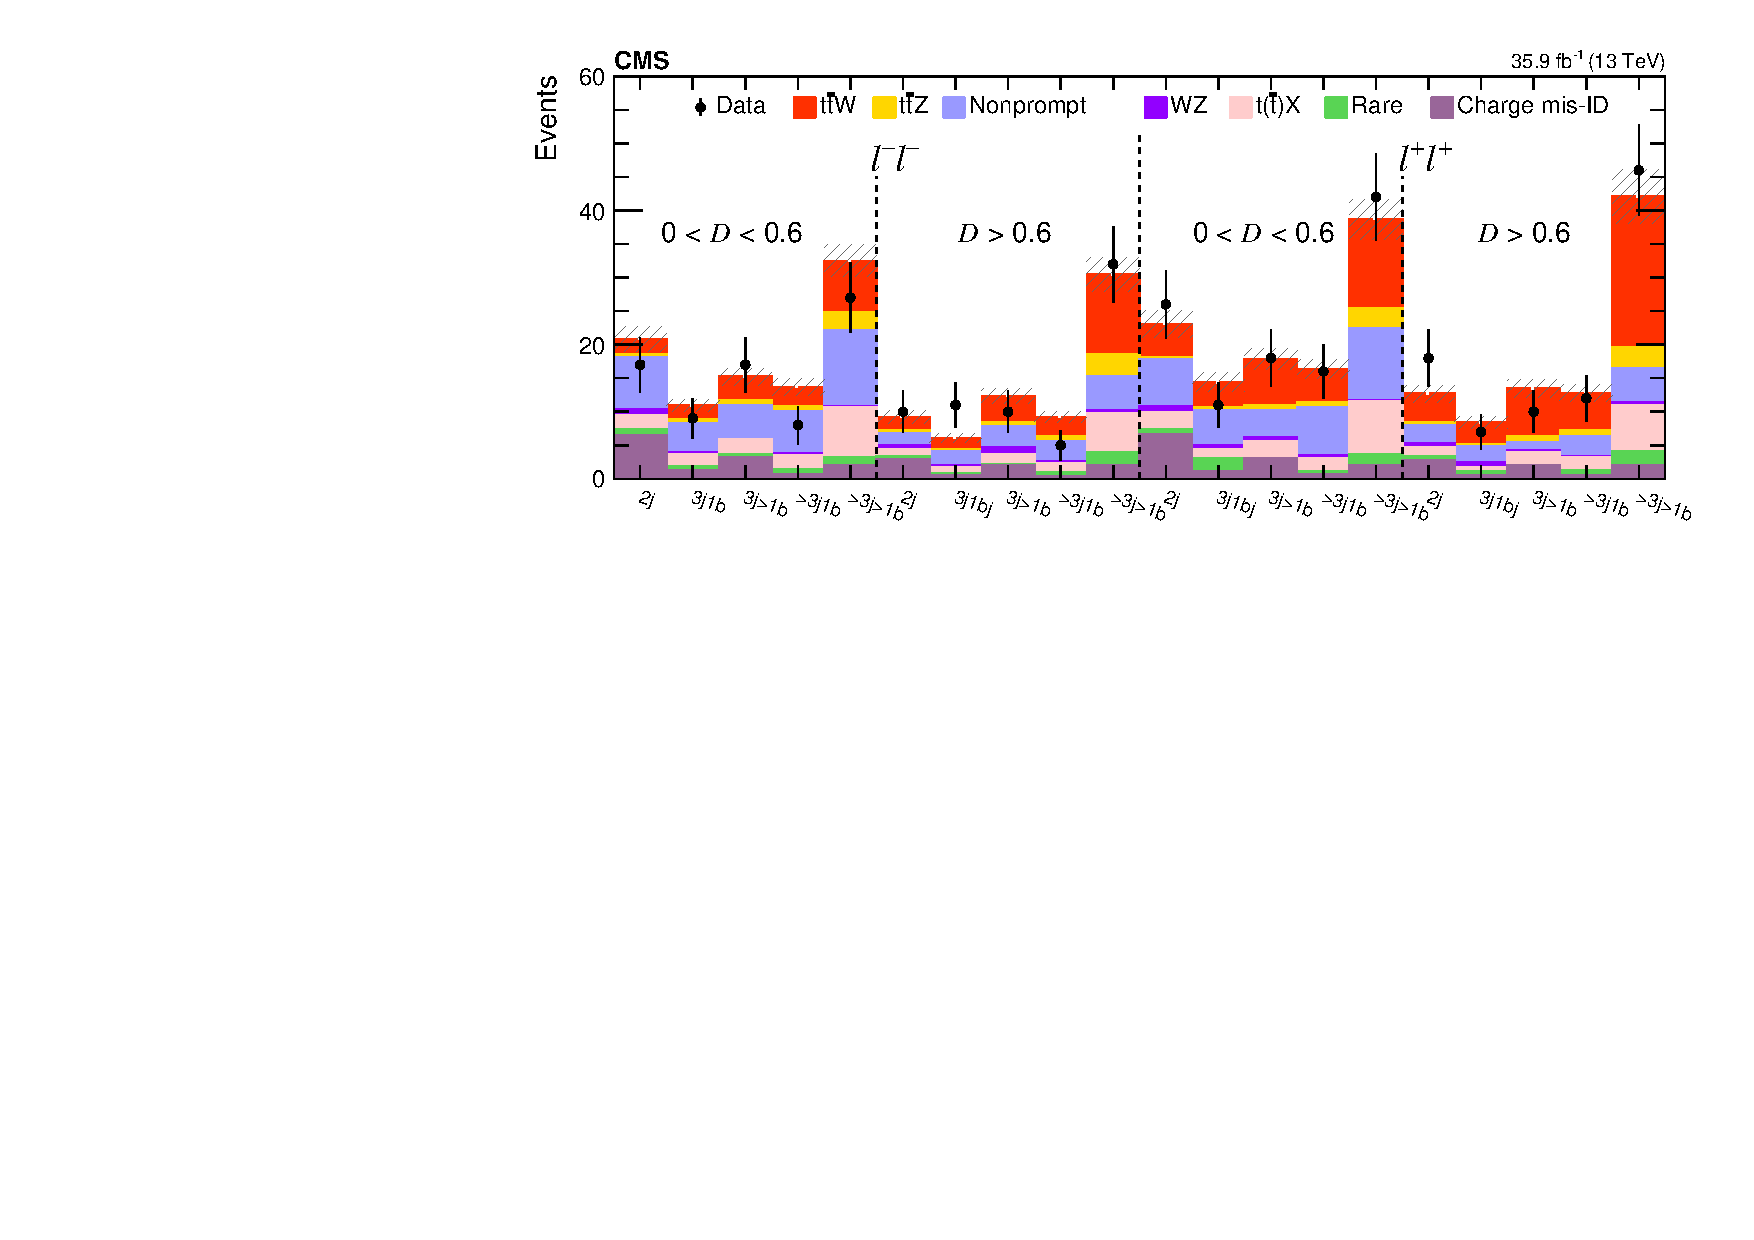
\includegraphics[width=\textwidth]{figures/thirteen-TeV/postfit-2lss}
  \caption[Post-fit yields for each category in the SS \ttW channel]{Predicted and observed post-fit
  yields for each category in the SS \ttW channel. The total post-fit uncertainty is shown as a
  hatched band.}
    \label{fig:13-postfit-ttW}
\end{figure}
\begin{figure}
  \centering
  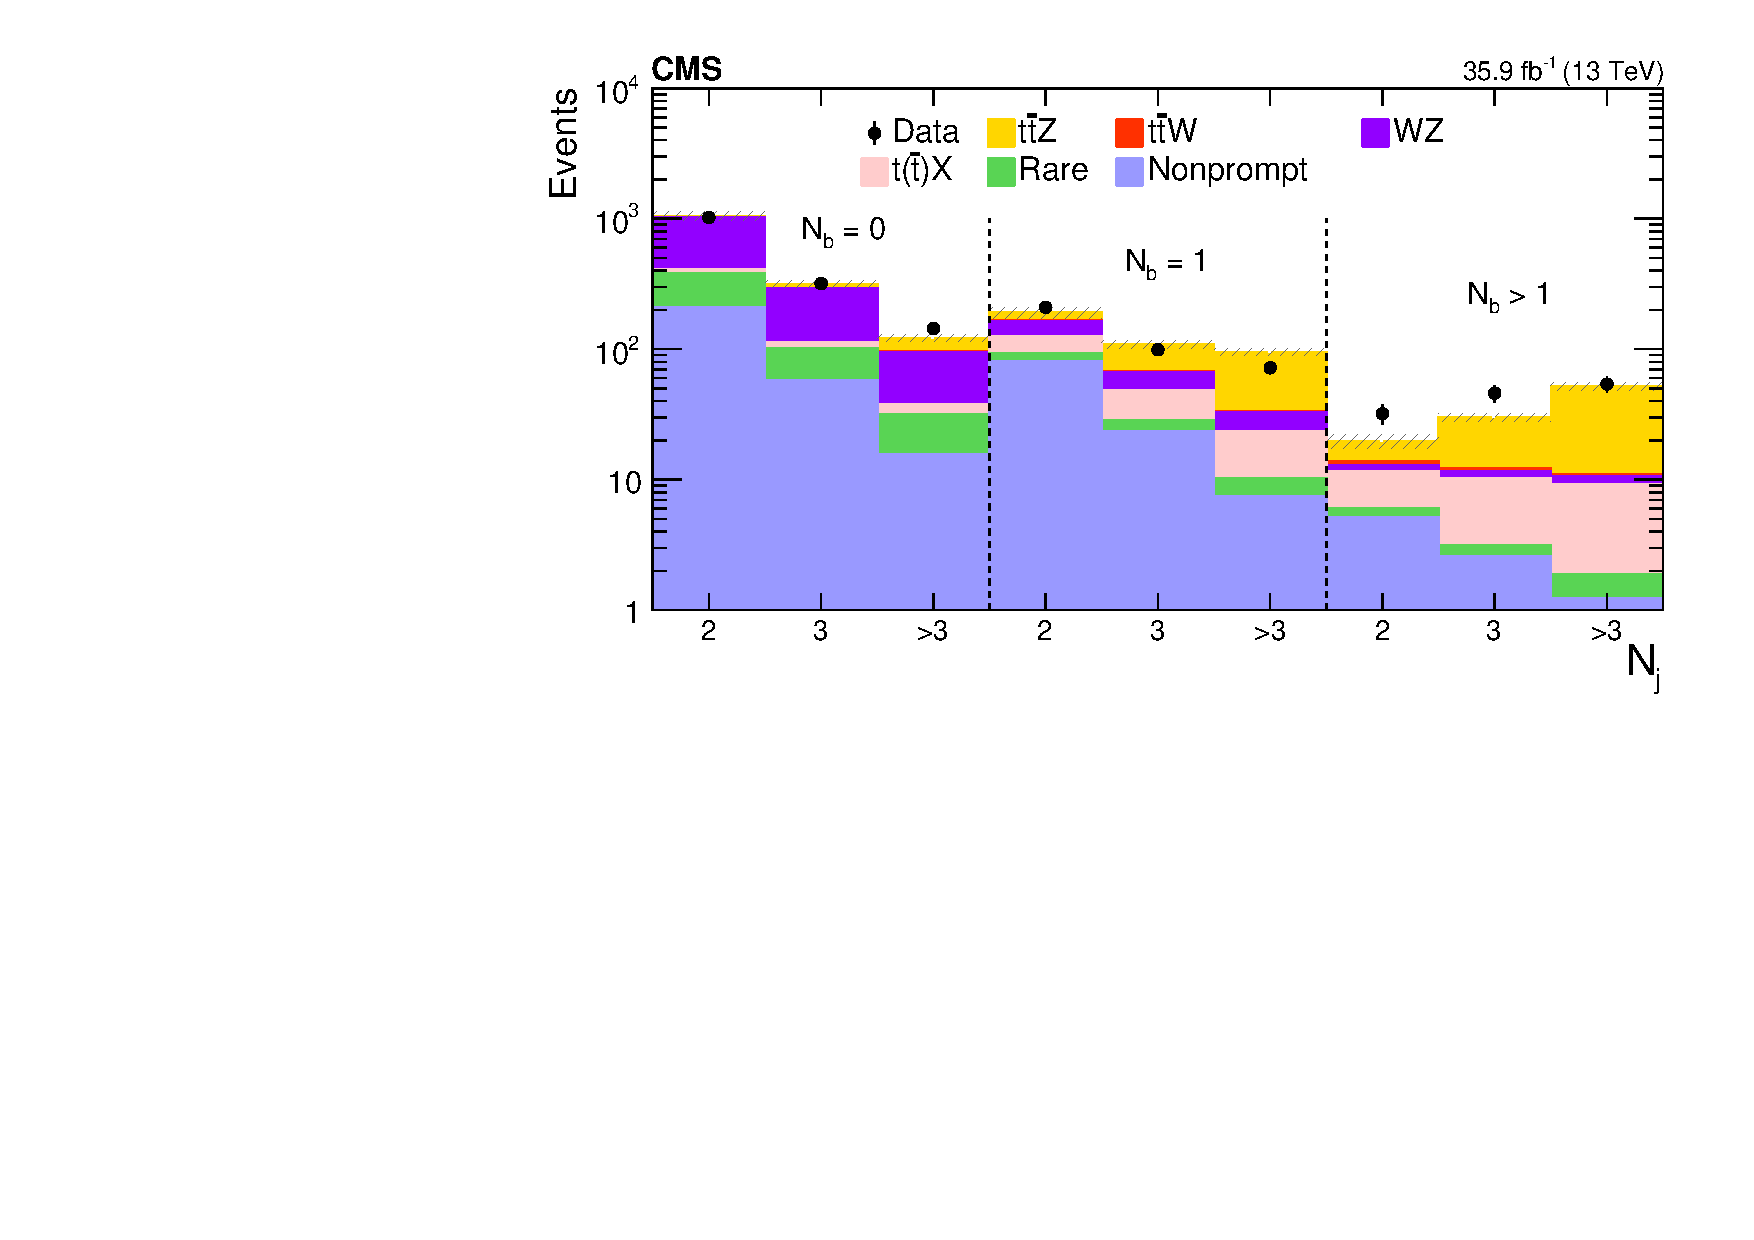
\includegraphics[width=0.66\textwidth]{figures/thirteen-TeV/postfit-3l}
  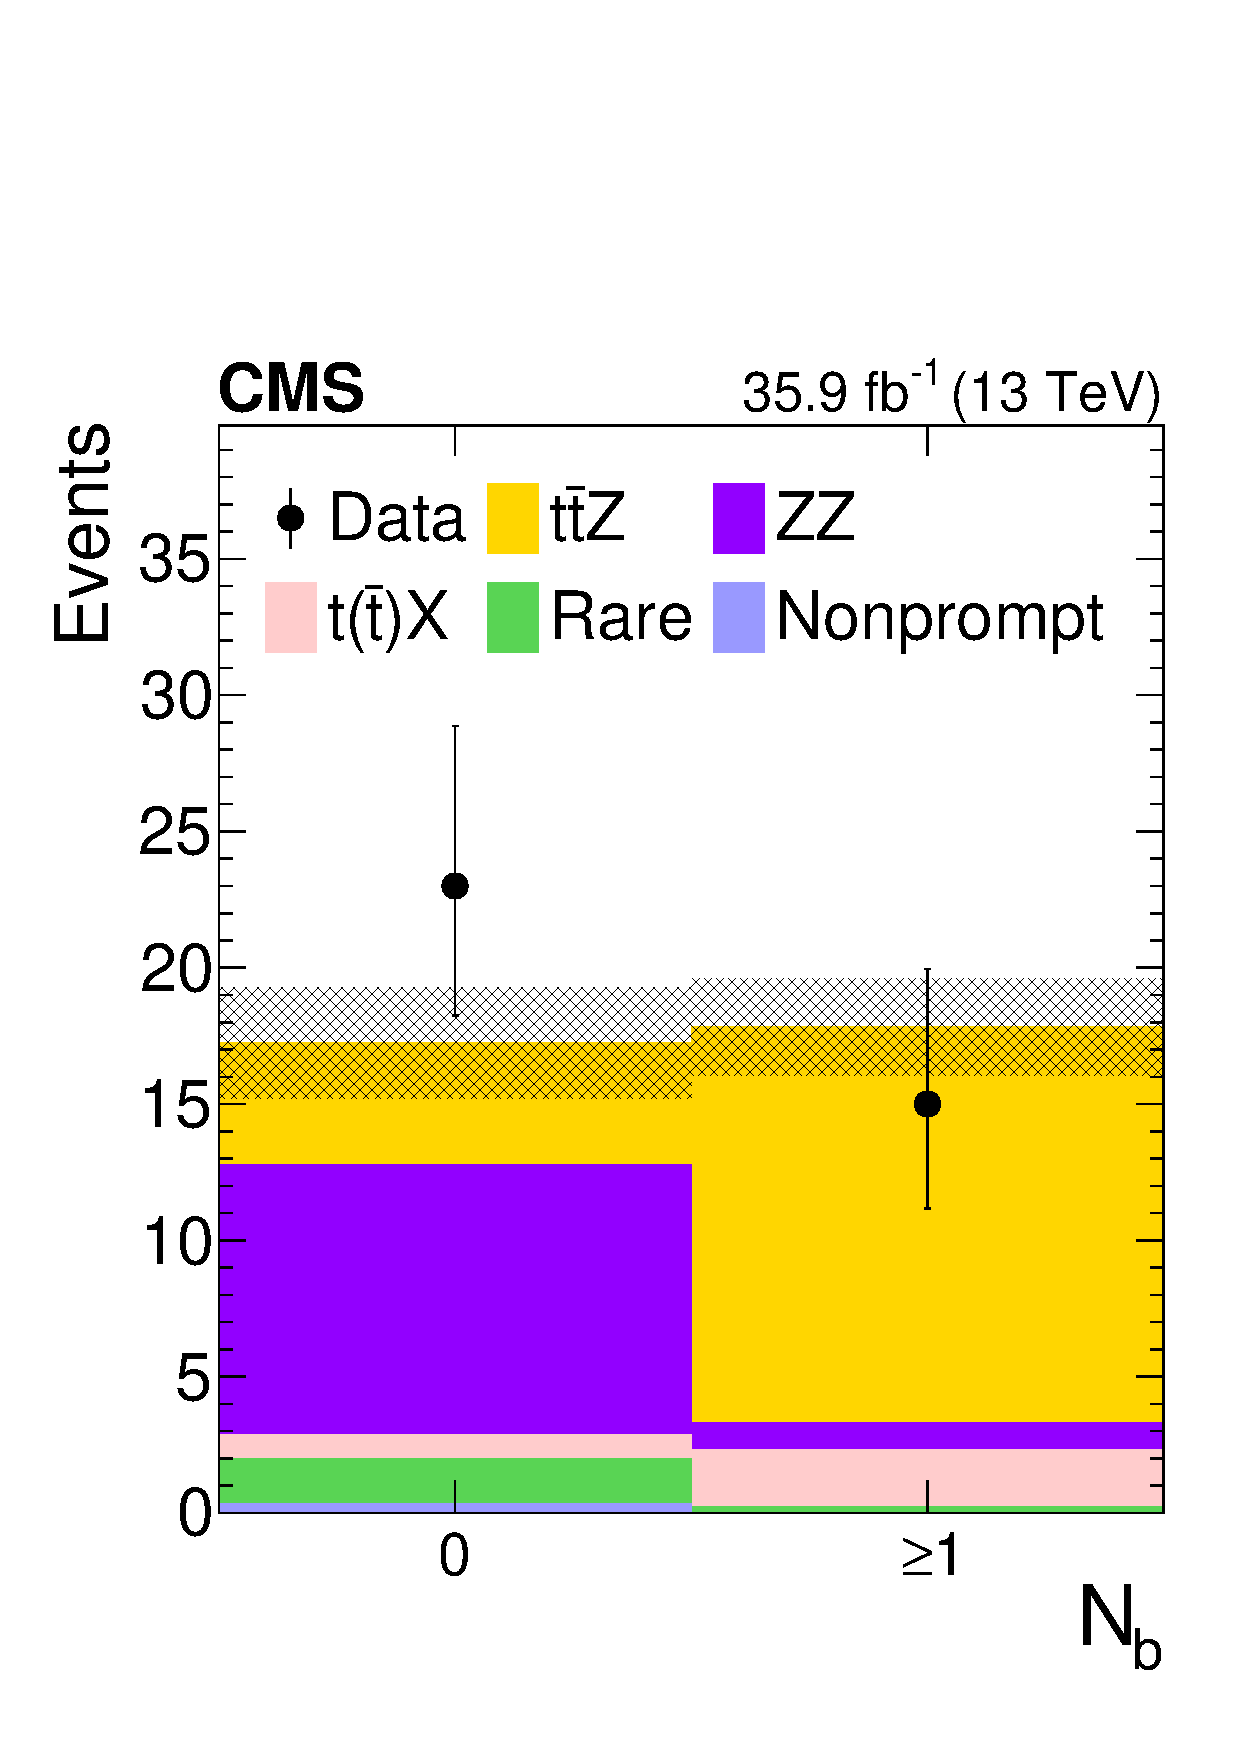
\includegraphics[width=0.32\textwidth]{figures/thirteen-TeV/postfit-4l}
  \caption[Post-fit yields for each category in the 3\lep \ttZ channel]{Predicted and observed post-fit yields for each category in the 3\lep \ttZ channel (left) and the 4\lep \ttZ channel (right). The total post-fit uncertainty is shown as a hatched band.}
  \label{fig:13-postfit-ttZ}
\end{figure}
\begin{table}
  \centering
  \caption{Post-fit yields for the SS \ttW channel ($D < 0$)}
  \label{tab:13-yields-2lss-CR}
  \input{tables/thirteen-TeV/yields-2lss-CR}
\end{table}
\begin{table}
  \centering
  \caption{Post-fit yields for the SS \ttW channel ($D > 0$)}
  \label{tab:13-yields-2lss-SR}
  \input{tables/thirteen-TeV/yields-2lss-SR}
\end{table}
\begin{table}
  \centering
  \caption{Post-fit yields for the 3\lep \ttZ channel}
  \label{tab:13-yields-3l}
  \input{tables/thirteen-TeV/yields-3l}
\end{table}
\begin{table}
  \centering
  \caption{Post-fit yields for the 4\lep \ttZ channel}
  \label{tab:13-yields-4l}
  \input{tables/thirteen-TeV/yields-4l}
\end{table}
\begin{table}
  \input{tables/thirteen-TeV/significances}
\end{table}
\begin{figure}
    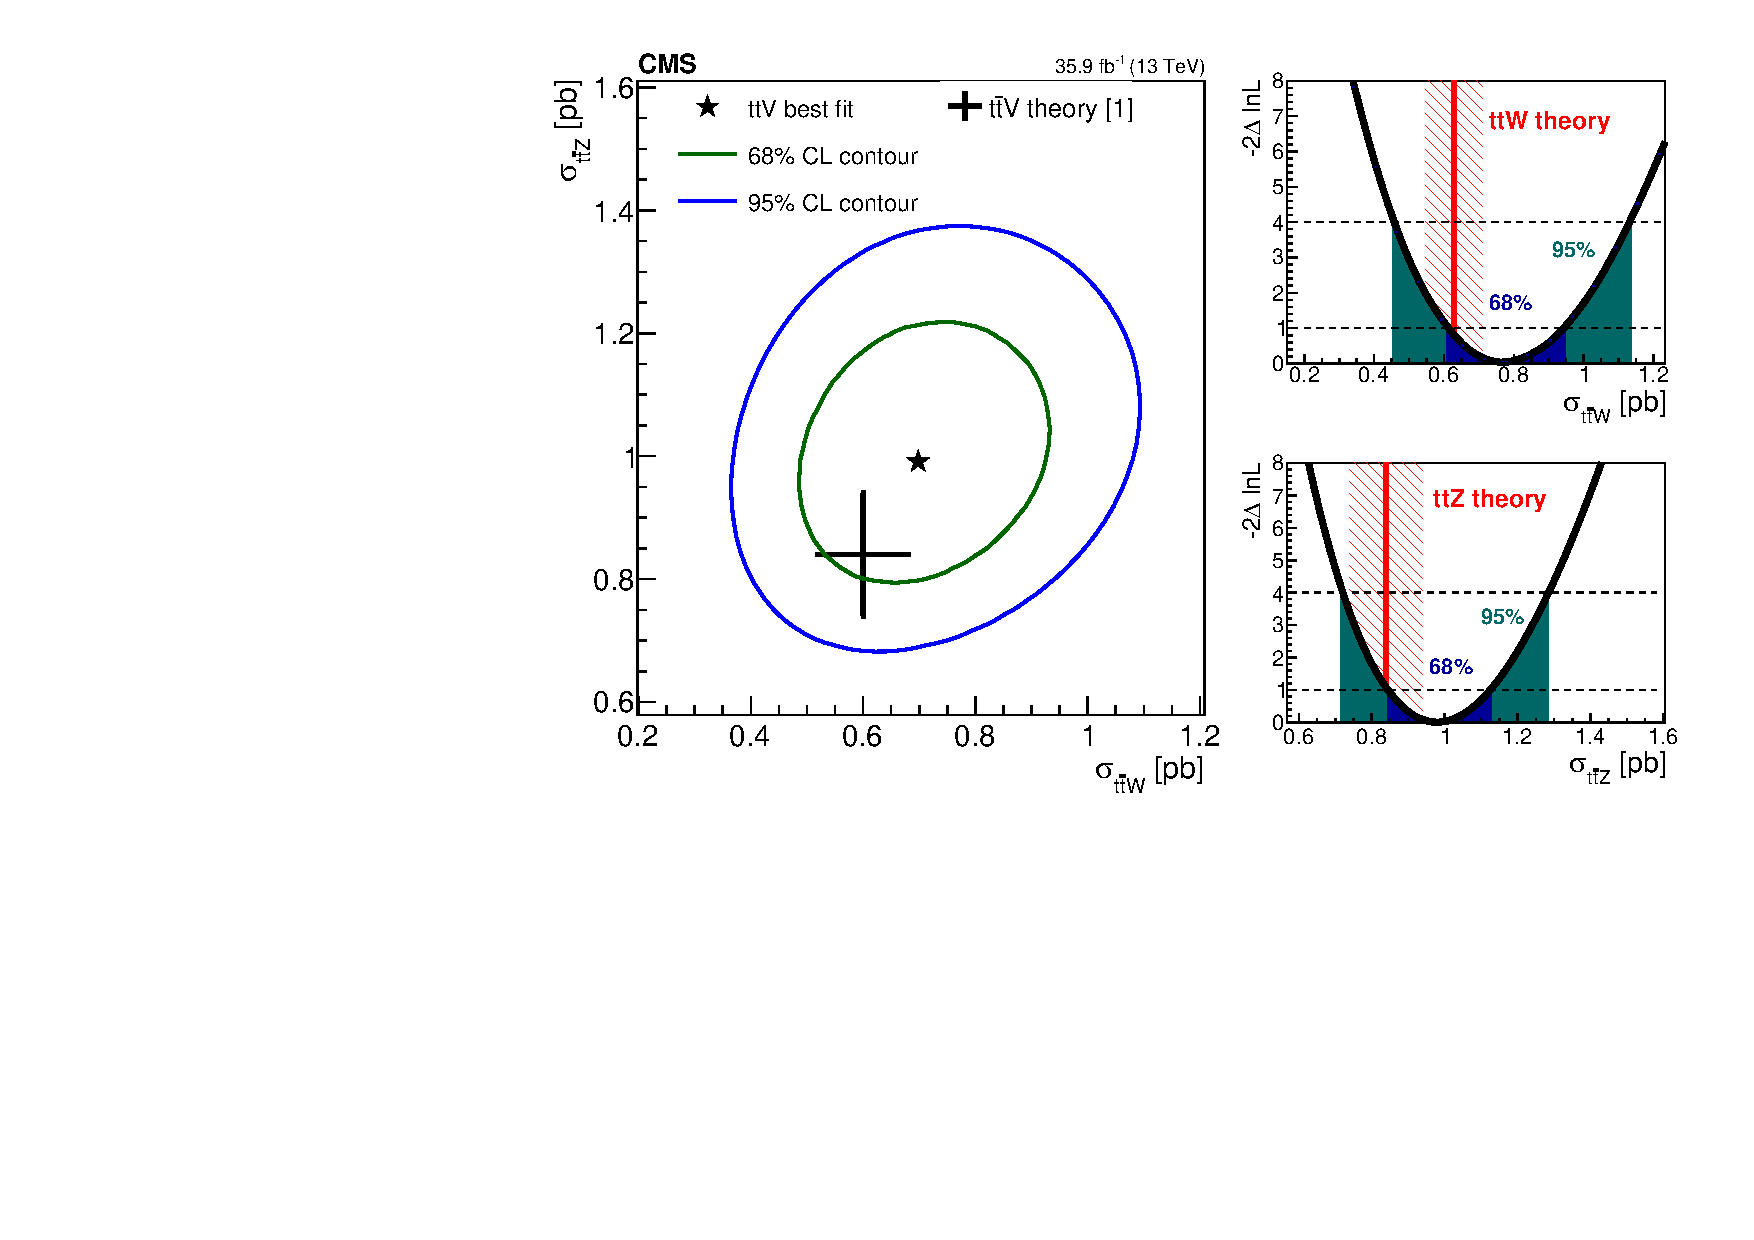
\includegraphics[width=0.90\textwidth]{figures/thirteen-TeV/sm-2d}
    \caption[Simultaneous fit for the \ttW and \ttZ cross sections]{Left: Result of the simultaneous fit for the \ttW and \ttZ cross sections, shown as a star, along with the corresponding 68 and \SI{95}{\percent} CL contours. Right: likelihood scan for the one-dimensional fit for \ttW (top) and \ttZ (bottom), along with the 68 and \SI{95}{\percent} CL intervals and the theory prediction~\cite{deFlorian:2016spz}.}
    \label{fig:13-sm-2d}
\end{figure}

